\title{Standard Matrices of Linear Transforms} 
\subtitle{\SubTitleName}
\institute[]{\Course}
\author{\Instructor}
\maketitle   

\frame{\frametitle{Topics and Learning Objectives}

\Emph{Topics} \\

\TopicStatement

\begin{itemize}
    \item the \Emph{standard vectors} and the \Emph{standard matrix}
    \item two dimensional transformations in more detail
    % \item \Emph{Onto} and \Emph{one-to-one} transformations. 
\end{itemize}

\vspace{0.5cm}
    
    \LO\\
    
    \LearningObjectiveStatement
    
    \begin{itemize}
        \item identify and construct linear transformations of a matrix
        % \item Characterize linear transformations as onto and/or one-to-one. 
        % \item Solve linear systems represented as linear transforms.
        % \item Express linear transforms in other forms, such as as matrix equations or as vector equations.
    \end{itemize}



\vspace{0.25cm} 

%\Emph{Motivating Question} \\

%A linear transformation  $ T \;:\;  \mathbb R ^2 \mapsto \mathbb R ^{3} $  satisfies 
%\begin{equation*}
%T \begin{pmatrix} 1 \\ 0 \end{pmatrix} = \begin{pmatrix} 5 \\ -7 \\ 2  \end{pmatrix},
%\qquad 
%T \begin{pmatrix*}[r]  0 \\ 1 \end{pmatrix*} = \begin{pmatrix*}[r] -3 \\ 8 \\ 0  
%\end{pmatrix*}
%\end{equation*}
%Is there a matrix that represents $ T_A$? If so, what could it be equal to? 
}






% \frame{\frametitle{Definition: The Standard Vectors}

%     The \Emph{standard vectors} in $\mathbb R^n$ are the vectors $\vec e_1, \vec e_2, \ldots , \vec e_n$, where: 
    
%     $$\vec e_1 = \hspace{2cm} \vec e_2 = \hspace{2cm} \vec e_n = $$
    
%     \vspace{2cm} 
    
%     For example, in $\mathbb R^3$, 
    
%         $$\vec e_1 = \hspace{2cm} \vec e_2 = \hspace{2cm} \vec e_3 = $$

% } 


% \frame{\frametitle{A Property of the Standard Vectors}

%     \Emph{Note}: if $A$ is an $m\times n$ matrix with columns $\vec v_1,\vec v_2,\ldots, \vec v_n$, then
%     $$A\vec e_i = \vec v_i, \text{ for } i=1,2,\ldots,n$$
%     So multiplying a matrix by $\vec e_i$ gives column $i$ of $A$.\\[6pt]

%     \Emph{Example}\\
%     $$\spalignmat{1 2 3; 4 5 6; 7 8 9} \vec e_2 = \hspace{6cm} $$

    
% }




% \frame{\frametitle{The Standard Matrix}

% \begin{center}\begin{tikzpicture} \node [mybox](box){\begin{minipage}{0.80\textwidth} 

%     Let $  T \;:\;  \mathbb R ^n \mapsto \mathbb R ^m $ be a linear transformation.  
%     Then there is a unique matrix $ A$ such that 
%     \begin{equation*}
%         T ( \vec x ) = A \vec x, \qquad \vec x\in \mathbb R ^{n}. 
%     \end{equation*}
%     In fact, $ A$ is a $ m \times n$, and its $ j^{th}$ column is the vector $ T (\vec e _j)$.  
%     \begin{equation*}
%         A = \begin{pmatrix}
%         T (\vec e_1) & T(\vec e_2)  & \cdots  & T (\vec e_n)
%     \end{pmatrix}
%     \end{equation*}

%     \end{minipage}}; \node[fancytitle, right=10pt] at (box.north west) {Theorem}; \end{tikzpicture}\end{center}

%     The matrix $ A$ is the \Emph{standard matrix} for a linear transformation.

% }



% \frame{\frametitle{Rotations}

%     \Emph{Example 1} \\
%     What is the linear transform $T : \R^2 \rightarrow \R^2$ defined by 
%     \begin{center}
%         $T(\vec x) = \vec x \text{ rotated counterclockwise by angle } \theta$?
%     \end{center}


% }

\frame{\frametitle{Standard Matrices in $\mathbb R^2$}

    \begin{itemize}
        \item There is a long list of geometric transformations of $\R^2$ in our textbook, as well as on the next few slides
        (reflections, rotations, contractions and expansions, shears, projections, \ldots).
        \item Please familiarize yourself with them: you are expected to memorize them, or be able to derive them.
    \end{itemize}

}



\frame{\frametitle{Two Dimensional Examples: Reflections}
    \vspace{-16pt}
    {\small 
    \begin{center}
        \begin{tabular}{ p{4.5cm} p{4.0cm} p{3.5cm}}
        \hline
        \Emph{transformation} & \Emph{image of unit square} & \Emph{standard matrix} \\
        \hline 
        \vspace{2pt} reflection through $x_1-$axis & 
        \vspace{2pt} \input{Chapter1/images/TransformReflectionX1.tex} & 
        \vspace{2pt} $\spalignmat{1 0;0 -1}$
        \\
        \vspace{2pt} reflection through $x_2-$axis & 
        \vspace{2pt} \input{Chapter1/images/TransformReflectionX2.tex} & 
        \vspace{2pt} $\spalignmat{-1 0;0 1}$
        \\        
        \end{tabular}
    \end{center}
    }
}

\frame{\frametitle{Two Dimensional Examples: Reflections}
    \vspace{-16pt}
    {\small 
    \begin{center}
        \begin{tabular}{ p{4.5cm} p{4.0cm} p{3.5cm}}
        \hline
        \Emph{transformation} & \Emph{image of unit square} & \Emph{standard matrix} \\
        \hline 
        \vspace{2pt} reflection through $x_2=x_1$ & 
        \vspace{2pt} 
        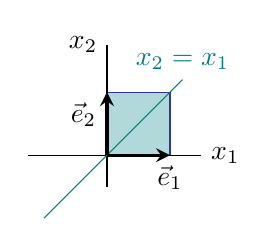
\begin{tikzpicture}[scale=0.8]

    \coordinate (O) at (0,0);  % variable for origin
       
    % grey and blue box
        \filldraw[
        draw=DarkBlue!80,fill=Teal!30]          
            (1,0) 
            -- (1,1)
            -- (0,1)
            -- (O)
            -- cycle;
            
          
    % axes
    \draw[-, thin,black] (-1.25,0) -- (1.5,0) node[anchor=west] {$x_1$};
    \draw[-, thin,black] (0,-0.5) -- (0.0,1.75) node[anchor=east] {$x_2$};
    
    % reflection line
    \draw[-,thin,Teal](-1,-1)--(1.2,1.2) node[anchor=south] {$x_2=x_1$};
    
    % coordinate vectors            
    \draw[->,Black,very thick,-stealth,rotate=0] (O) -- (0,1) node[anchor=north east] {$\vec e_2$}; 
    \draw[->,Black,very thick,-stealth,rotate=0] (O) -- (1,0) node[anchor=north] {$\vec e_1$}; 
    
\end{tikzpicture}&
        \vspace{2pt} $\spalignmat{0 1;1 0}$
        \\
        \vspace{2pt} reflection through $x_2=-x_1$ & 
        \vspace{2pt} 
        \input{Chapter1/images/Transformreflectionx2-x1.tex}&
        \vspace{2pt} $\spalignmat{0 -1;-1 0}$
        \\        
        \end{tabular}
    \end{center}
    }
}



\frame{\frametitle{Two Dimensional Examples: Contractions and Expansions}
    \vspace{-16pt}
    {\small 
    \begin{center}
        \begin{tabular}{ p{4.5cm} p{3.4cm} p{4cm}}
        \hline
        \Emph{transformation} & \Emph{image of unit square} & \Emph{standard matrix} \\
        \hline 
        \vspace{2pt} horizontal contraction & 
        \vspace{2pt} 
        \input{Chapter1/images/HorizontalContraction.tex}&
        \vspace{2pt} $\spalignmat{k 0;0 1}$. $|k|<1$
        \\
        \vspace{2pt} horizontal expansion & 
        \vspace{2pt} 
        \input{Chapter1/images/HorizontalExpansion.tex}&
        \vspace{2pt} $\spalignmat{k 0;0 1}$, $k>1$
        \\        
        \end{tabular}
    \end{center}
    }
}

\frame{\frametitle{Two Dimensional Examples: Contractions and Expansions}
    \vspace{-16pt}
    {\small 
    \begin{center}
        \begin{tabular}{ p{4.5cm} p{3.4cm} p{4cm}}
        \hline
        \Emph{transformation} & \Emph{image of unit square} & \Emph{standard matrix} \\
        \hline 
        \vspace{2pt} vertical contraction & 
        \vspace{2pt} 
        \input{Chapter1/images/VerticalContraction.tex}&
        \vspace{2pt} $\spalignmat{1 0;0 k}$, $|k|<1$
        \\
        \vspace{2pt} vertical expansion & 
        \vspace{2pt} 
        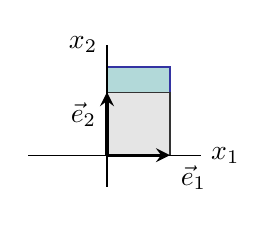
\begin{tikzpicture}[scale=0.8]

    \coordinate (O) at (0,0);  % variable for origin

    % blue box
        \filldraw[
        draw=DarkBlue!80,fill=Teal!30]          
            (1,0) 
            -- (1,1.4)
            -- (0,1.4)
            -- (O)
            -- cycle;                
    % grey box
        \filldraw[
        draw=black!80,fill=black!10]          
            (0,1) 
            -- (1,1)
            -- (1,0)
            -- (O)
            -- cycle;
            
        
    % axes
    \draw[-, thin,black] (-1.25,0) -- (1.5,0) node[anchor=west] {$x_1$};
    %\draw[.,thin,black] (1,0) node[anchor=north]{$k>1$};
    \draw[-, thin,black] (0,-0.5) -- (0.0,1.75) node[anchor=east] {$x_2$};
    
    % coordinate vectors                
    \draw[->,Black,very thick,-stealth,rotate=0] (O) -- (0,1) node[anchor=north east] {$\vec e_2$}; 
    \draw[->,Black,very thick,-stealth,rotate=0] (O) -- (1,0) node[anchor=north west] {$\vec e_1$}; 
    
        
\end{tikzpicture}&
        \vspace{2pt} $\spalignmat{1 0;0 k}$, $k>1$
        \\        
        \end{tabular}
    \end{center}
    }
}


\frame{\frametitle{Two Dimensional Examples: Shears}
    \vspace{-8pt}
    {\small 
    \begin{center}
        \begin{tabular}{ p{4.5cm} p{3.4cm} p{4cm}}
        \hline
        \Emph{transformation} & \Emph{image of unit square} & \Emph{standard matrix} \\
        \hline 
        \vspace{2pt} horizontal shear (left) & 
        \vspace{2pt} 
        \input{Chapter1/images/Horizontalshearleft.tex}&
        \vspace{2pt} $\spalignmat{1 k;0 1}$, $k<0$
        \\
        \vspace{2pt} horizontal shear (right) & 
        \vspace{2pt} 
        \input{Chapter1/images/Horizontalshearright.tex}&
        \vspace{2pt} $\spalignmat{1 k;0 1}$, $k>0$
        \\        
        \end{tabular}
    \end{center}
    }
}



\frame{\frametitle{Two Dimensional Examples: Shears}
    \vspace{-8pt}
    {\small 
    \begin{center}
        \begin{tabular}{ p{4.5cm} p{4.0cm} p{3.5cm}}
        \hline
        \Emph{transformation} & \Emph{image of unit square} & \Emph{standard matrix} \\
        \hline 
        \vspace{2pt} vertical shear (down) & 
        \vspace{2pt} 
        \input{Chapter1/images/Verticalsheardown.tex}&
        \vspace{2pt} $\spalignmat{1 0;k 1}$, $k<0$
        \\
        \vspace{2pt} vertical shear (up) & 
        \vspace{2pt} 
        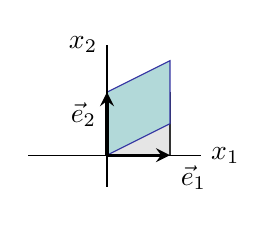
\begin{tikzpicture}[scale=0.8]

    \coordinate (O) at (0,0);  % variable for origin

    % grey box
        \filldraw[
        draw=black!80,fill=black!10]          
            (0,1) 
            -- (1,1)
            -- (1,0)
            -- (O)
            -- cycle;
            
    % blue box
        \filldraw[
        draw=DarkBlue!80,fill=Teal!30]          
            (0,1) 
            -- (1,1.5)
            -- (1,0.5)
            -- (0,0)
            -- cycle;            
    % axes
    \draw[-, thin,black] (-1.25,0) -- (1.5,0) node[anchor=west] {$x_1$};
    %\draw[., thin,black] (1,0) node[anchor=north]{$k>0$};
    \draw[-, thin,black] (0,-0.5) -- (0.0,1.75) node[anchor=east] {$x_2$};
    
    % coordinate vectors                
    \draw[->,Black,very thick,-stealth,rotate=0] (O) -- (0,1) node[anchor=north east] {$\vec e_2$}; 
    \draw[->,Black,very thick,-stealth,rotate=0] (O) -- (1,0) node[anchor=north west] {$\vec e_1$}; 
    
        
\end{tikzpicture}&
        \vspace{2pt} $\spalignmat{1 0;k 1}$, $k>0$
        \\        
        \end{tabular}
    \end{center}
    }
}



\frame{\frametitle{Two Dimensional Examples: Projections}
    \vspace{-8pt}
    {\small 
    \begin{center}
        \begin{tabular}{ p{4.5cm} p{4.0cm} p{3.5cm}}
        \hline
        \Emph{transformation} & \Emph{image of unit square} & \Emph{standard matrix} \\
        \hline 
        \vspace{2pt} projection onto the $x_1$-axis & 
        \vspace{2pt} 
        \input{Chapter1/images/Projectionx1.tex}&
        \vspace{2pt} $\spalignmat{1 0;0 0}$
        \\
        \vspace{2pt} projection onto the $x_2$-axis & 
        \vspace{2pt} 
        \input{Chapter1/images/Projectionx2.tex}&
        \vspace{2pt} $\spalignmat{0 0;0 1}$
        \\        
        \end{tabular}
    \end{center}
    }
}






\frame{\frametitle{Example: Composite Transform}

Construct a matrix $A \in \mathbb R^{2\times 2}$, such that $T(\vec{x}) = A\vec{x}$, where $T$ is a linear transformation that rotates vectors in $\mathbb R^2$ counterclockwise by $\pi/2$ radians about the origin, then reflects them through the line $x_1 = x_2$.

}



\frame{\frametitle{Summary}

    \SummaryLine \vspace{4pt}
    \begin{itemize}\setlength{\itemsep}{8pt}
            \item constructing linear transformations in $\mathbb R^2$ and gave geometric interpretations for them
            \item constructing composite transform that involve two ore more linear transforms
    \end{itemize}

}

